\documentclass[11pt,a4paper]{ctexart}
\usepackage[margin=1.8cm]{geometry}
\usepackage{amsmath,amssymb,bm}
\usepackage{booktabs,graphicx,xcolor,hyperref,array,float,tabularx}
\hypersetup{colorlinks=true,linkcolor=blue,urlcolor=blue,citecolor=blue}
\setlength{\parindent}{2em}
\setlength{\parskip}{0.22em}
\newcommand{\Exp}{\operatorname{Exp}}
\newcommand{\norm}[1]{\left\lVert #1\right\rVert}
\title{只关心位置时，IMU--UWB InEKF 是否多余？}
\author{状态耦合、原论文目标与当前数据复核}
\date{2026年8月3日}

\begin{document}
\pagestyle{plain}
\maketitle

\begin{abstract}
本项目的主要交付指标可以是位置，但当前估计模型并非“无姿态问题”。机体系
加速度必须经姿态旋到世界系，UWB标签的非零杆臂也使TDoA预测依赖姿态。
因此姿态是位置估计的隐变量，不能因为下游不输出姿态就直接删除。另一方面，
公平ESKF--15同样包含姿态、速度、位置和IMU偏置；InEKF的额外价值是群上一致
误差与较大的有效线性化范围，而不是增加了一个ESKF不需要的状态。原论文主要
证明180度初始航向下姿态收敛改善，并明确两者位置、速度相近。当前const1前
30 s复核中，180度相对0度初始yaw使位置RMSE由$0.107016$ m增至
$0.111630$ m（$+4.31\%$），两次均无UWB拒绝且轨迹连续。故本项目保留姿态
状态和InEKF有合理性，但“InEKF相对公平ESKF对纯位置任务必不可少”尚需同协议
基线证明。
\end{abstract}

\section{先区分两个命题}

“最终只关心位置”和“滤波模型不涉及姿态”不是同一件事。当前工程状态为
\begin{equation}
 \delta x=\begin{bmatrix}
 \delta\theta^\top&\delta v^\top&\delta p^\top&
 \delta b_g^\top&\delta b_a^\top
 \end{bmatrix}^\top\in\mathbb R^{15},
 \label{eq:error-state}
\end{equation}
名义导航状态写成
\begin{equation}
 X=\begin{bmatrix}R&v&p\\0&1&0\\0&0&1\end{bmatrix}
 \in SE_2(3).
 \label{eq:se23}
\end{equation}
公平ESKF--15也需要式~\eqref{eq:error-state}中的同一组物理状态。二者的核心
差别是误差定义、线性化坐标和状态注入，不是InEKF多估计了一个下游不用的量。

所以本问题应改写为：姿态是否是位置的必要隐变量，以及使用不变误差是否比普通
误差状态在目标工况下更稳健。

\section{姿态为何进入位置模型}

\subsection{机体系IMU使传播不能只写成位置--速度闭环}

当前离散传播的基本结构为
\begin{align}
 R_{k+1}&=R_k\Exp\big((\omega_{m,k}-b_{g,k})\Delta t\big),\\
 v_{k+1}&=v_k+\left(R_k(a_{m,k}-b_{a,k})+g\right)\Delta t,\\
 p_{k+1}&=p_k+v_k\Delta t
 +\frac12\left(R_k(a_{m,k}-b_{a,k})+g\right)\Delta t^2.
 \label{eq:mechanization}
\end{align}
若$\delta\theta$很小，世界系加速度的一阶误差为
\begin{equation}
 \delta a^w\simeq-R[a_m-b_a]_\times\delta\theta.
 \label{eq:attitude-to-acc}
\end{equation}
在重力主导时，$1^\circ$ roll/pitch误差对应约
$9.81\times\pi/180=0.171\ {\rm m/s^2}$水平伪加速度；1 s内仅二次积分项
即可产生约$0.086$ m位置误差。yaw在静止重力下弱可观，但水平机动时会旋错
水平比力，仍会传导到位置。

只有外部AHRS已给出可靠$R_k$及协方差、加速度已在世界系，或载体受严格固定姿态
约束时，才可把式~\eqref{eq:mechanization}降成独立位置--速度滤波器。直接把未知
姿态固定为单位阵会低估位置不确定度。

\subsection{非零UWB杆臂使量测也依赖姿态}

当前UWB标签相对机体参考点的标定为
\begin{equation}
 t_{uv}=\begin{bmatrix}-0.01245&0.00127&0.0908\end{bmatrix}^\top {\rm m},
 \qquad \norm{t_{uv}}=0.09166\ {\rm m}.
\end{equation}
因而TDoA预测为
\begin{equation}
 h_{BA}(R,p)=
 \norm{p+Rt_{uv}-a_B}-\norm{p+Rt_{uv}-a_A}.
 \label{eq:tdoa-lever}
\end{equation}
即使不使用IMU传播，式~\eqref{eq:tdoa-lever}也不是纯$p$量测。当前成熟路径的
名义预测保留$Rt_{uv}$；研究版完整杆臂姿态Jacobian只在\texttt{verified}模式
开启，生产路径则沿用经Adjoint变换的稳定量测坐标。这一边界必须如实说明，但它
不改变“名义量测依赖姿态”的事实。

\section{InEKF的价值与边界}

对无偏群仿射导航主块，右不变误差可使线性化误差动力学较少依赖当前名义轨迹，
并以$SE_2(3)$群乘法注入修正。相比在错误姿态附近直接作局部欧氏线性化，这通常
扩大大初始航向误差下的有效收敛域。因此InEKF的合理卖点是\textbf{姿态作为隐变量
时的位置鲁棒性和一致性}，而不是“只要换成InEKF，位置RMSE必然下降”。

当前系统仍有以下限制：
\begin{itemize}
 \item 偏置增广后，误差矩阵仍含$R,v,p$的偏置耦合；
 \item TDoA距离差仍是非线性量测，不会自动获得全局线性观测；
 \item 单标签静止yaw弱可观，必须依赖运动激励和惯性--位置耦合；
 \item 采用不变误差不能消除NLOS、错误门限、错误时间对齐或不可观测模态；
 \item 原论文承认InEKF增加计算资源，目标硬件仍需单独测WCET。
\end{itemize}

当前工程相对原论文公开实现已统一$[\theta,v,p,b_g,b_a]$顺序，修复SO(3)数值，
把物理先验映射到右不变协方差坐标，在一致坐标中计算UWB NIS，并用2 rad表示未知
全圆yaw。上述改进避免大yaw压力下的错误门控闭锁，但并不能替代公平ESKF基线。

\section{与原论文目标的对照}

原论文摘要、引言和结论均把问题定义为Crazyflie初始heading错误造成姿态收敛过慢。
论文给出的180度初始航向对比约为InEKF heading RMS $0.08$ rad、参考ESKF
$1.34$ rad；同时对其Figure 4的文字解释是两种滤波器的位置、速度RMS相近，主要
差异出现在姿态恢复。

\begin{table}[H]
\centering
\caption{原论文证据与“纯位置目标”的关系}
\begin{tabularx}{\textwidth}{p{3.0cm}X X}
\toprule
项目 & 原论文主要结论 & 对本问题的含义\\
\midrule
姿态/heading & 大初始yaw时InEKF显著快于ESKF & 支持InEKF处理大姿态初差\\
位置/速度 & 两者整体相近 & 不足以证明纯位置精度必然受益\\
计算 & InEKF需要更多资源 & 若无鲁棒性收益，简化有价值\\
状态模型 & $R,v,p$在$SE_2(3)$上联合估计 & 姿态本就是惯性位置传播的一部分\\
\bottomrule
\end{tabularx}
\end{table}

因此，若新项目排除姿态指标、初始姿态扰动、快速机动和失锁恢复，却仍把“InEKF”
本身作为主要贡献，容易出现目标与方法错位。更合理的表述是考察大姿态不确定性是否
通过隐变量耦合影响位置失效率、恢复时间和一致性。

\section{当前数据的受控复核}

使用指定Conda环境和当前\texttt{task03\_compiled}方程，对
\texttt{const1-trial1-tdoa2}前30 s运行0度与180度初始yaw。除初始yaw外，
数据、初始位置、roll/pitch、噪声、偏置初始化和UWB门限完全相同。

\begin{table}[H]
\centering
\caption{只改变初始yaw的当前InEKF结果}
\begin{tabular}{lrrrrr}
\toprule
初始yaw & 位置/m & 速度/(m/s) & 姿态/rad & yaw/rad & 拒绝\\
\midrule
$0^\circ$   & 0.107016 & 0.072891 & 0.157598 & 0.157491 & 0/14289\\
$180^\circ$ & 0.111630 & 0.075372 & 0.222601 & 0.222155 & 0/14289\\
相对变化 & $+4.31\%$ & $+3.40\%$ & $+41.25\%$ & $+41.06\%$ & 0\\
\bottomrule
\end{tabular}
\end{table}

\begin{figure}[H]
\centering
\begin{minipage}[t]{0.49\textwidth}
 \centering
 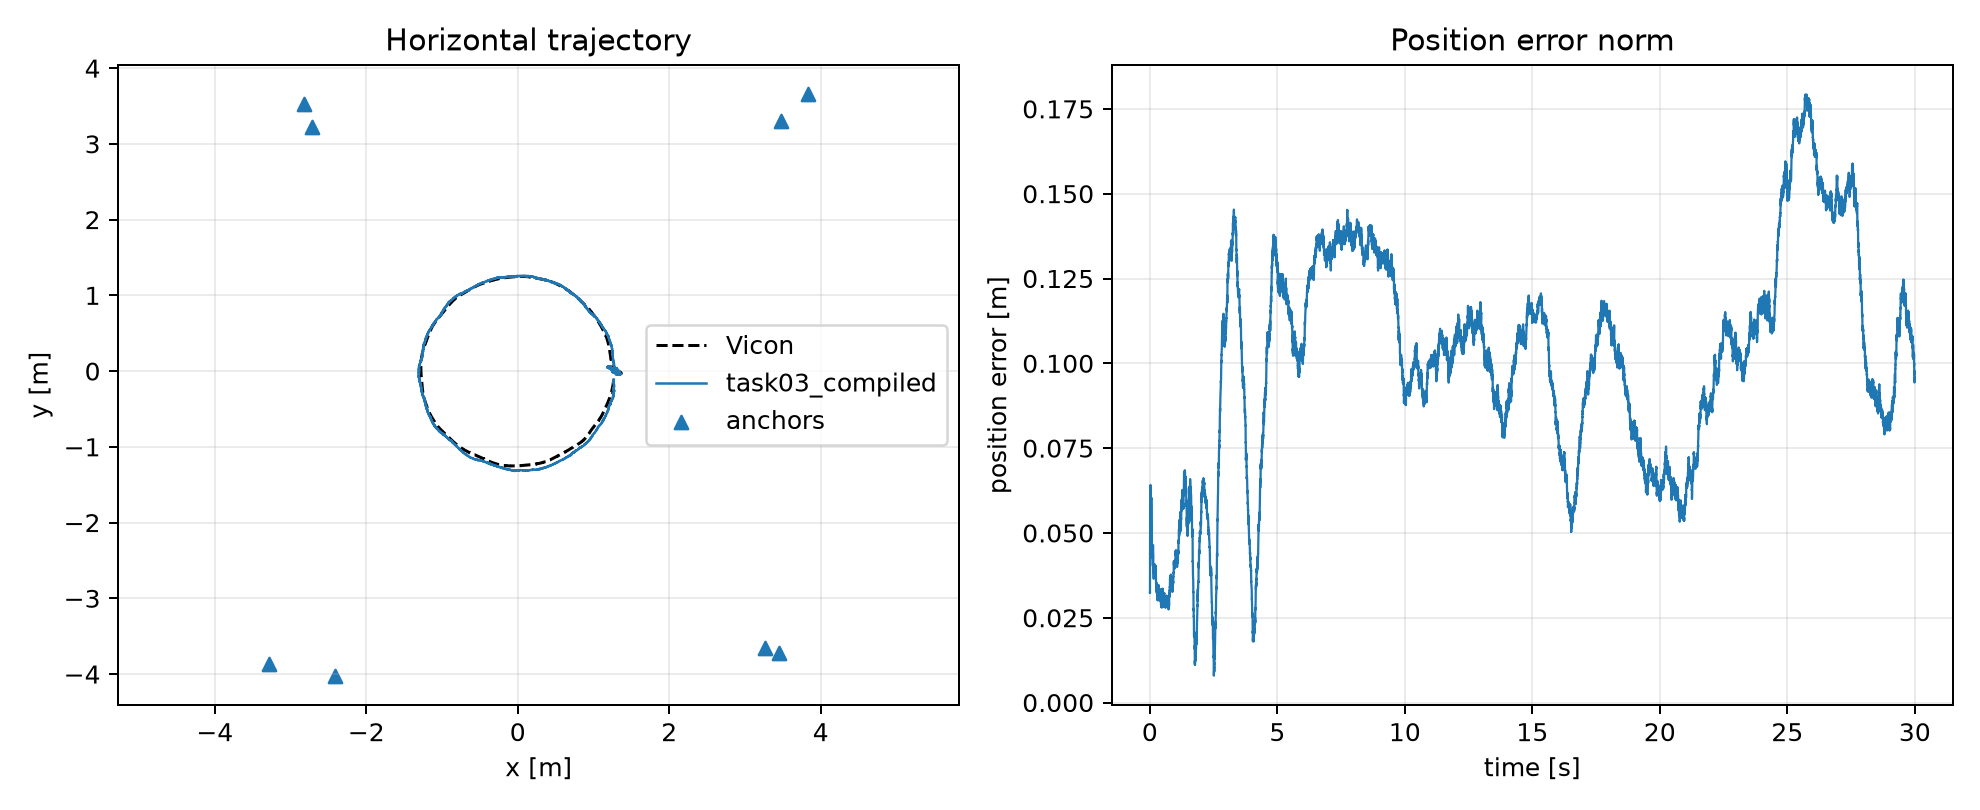
\includegraphics[width=\linewidth]{../imu-uwb-inekf/results/attitude_necessity_const1_yaw000/trajectory_and_position_error.png}
 \small (a) 初始yaw误差$0^\circ$
\end{minipage}
\hfill
\begin{minipage}[t]{0.49\textwidth}
 \centering
 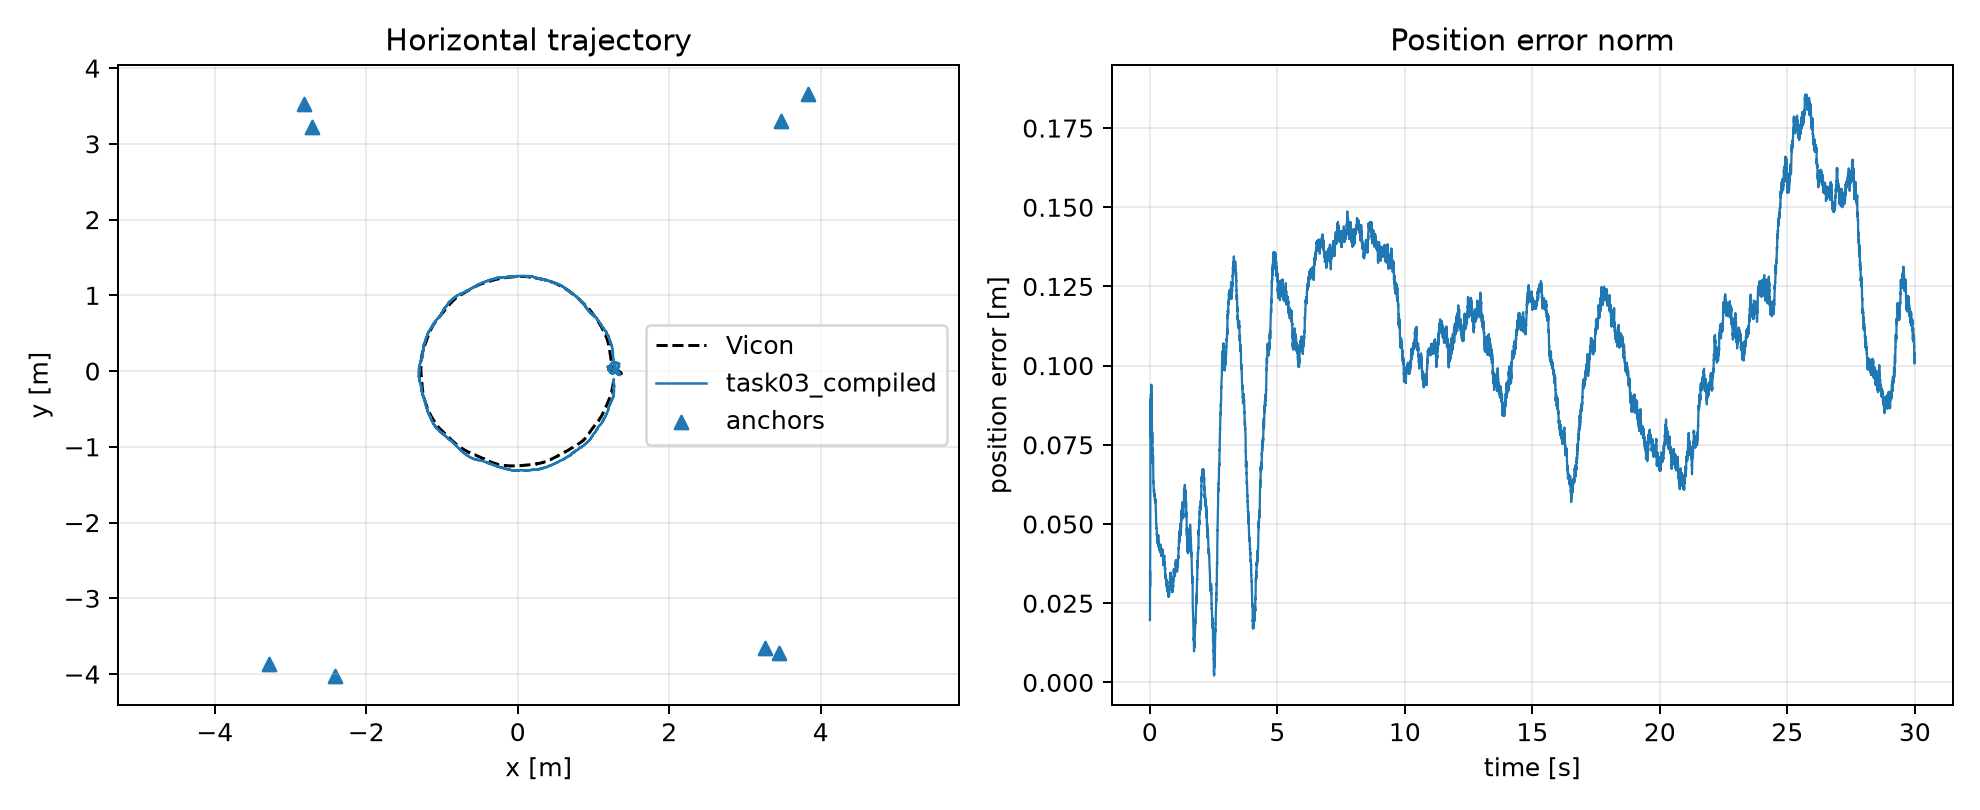
\includegraphics[width=\linewidth]{../imu-uwb-inekf/results/attitude_necessity_const1_yaw180/trajectory_and_position_error.png}
 \small (b) 初始yaw误差$180^\circ$
\end{minipage}
\caption{两组水平轨迹和位置误差。均连续、贴近Vicon且无发散。}
\label{fig:position}
\end{figure}

180度初差在启动后迅速降到约20度以内，但30 s内未持续进入5度；位置RMSE仅增加
约4.31\%。两次NIS均远低于25且没有拒绝差异。这说明姿态误差会传导到位置，同时
也说明在该温和轨迹上，InEKF的突出作用是限制大姿态初差的后果，而不是大幅改善
位置均方误差。

\section{何时InEKF可能确实是多余的}

\begin{table}[H]
\centering
\caption{按物理条件而非输出字段选择滤波器}
\begin{tabularx}{\textwidth}{p{4.2cm}p{3.1cm}X}
\toprule
条件 & 姿态状态 & 建议\\
\midrule
六自由度、机体系IMU、未知初始yaw & 必须估计 & InEKF合理，需和ESKF--15公平比较\\
可靠外部AHRS并提供姿态协方差 & 可作为外部输入 & 位置--速度EKF可行，须传播姿态不确定度\\
严格平面、固定航向且已验证 & 可降维 & 2D/3D简化EKF可能更合适\\
纯UWB高频定位、不需短时惯性传播 & 不需要 & 多边定位加运动滤波可作为基线\\
仅离线轨迹、允许全批处理 & 取决于模型 & 可考虑因子图/平滑器而非在线InEKF\\
\bottomrule
\end{tabularx}
\end{table}

当前UTIL Crazyflie数据包含倾斜、转向、快速手动机动和UWB异步量测，不满足可安全
固定姿态的条件。因此不能从“下游只读位置”直接推出“删除姿态或InEKF”。

\section{需要补齐的决定性实验}

当前仓库只有旧9维无偏置ESKF，不能用来决定InEKF是否值得。最小公平协议应为：
\begin{enumerate}
 \item 实现与当前InEKF同状态、同偏置、同IMU积分、同杆臂、同门限和同初始化的
 ESKF--15；
 \item 增加外部真值姿态输入的位置滤波器作为oracle上界，仅分解姿态代价；
 \item 增加纯UWB位置--速度基线，量化IMU贡献；
 \item 固定参数后覆盖0/90/180度初始yaw、自动/手动轨迹、UWB降频和NLOS；
 \item 以位置RMSE、最大误差、失败率、恢复时间、NIS/NEES和目标硬件WCET作主判据。
\end{enumerate}

在完成该对比前，最终结论应限定为：\textbf{姿态状态对当前位置模型不是多余的；
InEKF是合理选择，但它相对公平ESKF对纯位置目标的必要性尚未被当前项目单独证明。}

\end{document}

